% ! TeX program = xelatex


% Options for packages loaded elsewhere
\PassOptionsToPackage{unicode}{hyperref}
\PassOptionsToPackage{hyphens}{url}
%
\documentclass[
  ignorenonframetext,
]{beamer}
\usepackage{pgfpages}
\setbeamertemplate{caption}[numbered]
\setbeamertemplate{caption label separator}{: }
\setbeamercolor{caption name}{fg=normal text.fg}
\beamertemplatenavigationsymbolsempty
% Prevent slide breaks in the middle of a paragraph
\widowpenalties 1 10000
\raggedbottom
\setbeamertemplate{part page}{
  \centering
  \begin{beamercolorbox}[sep=16pt,center]{part title}
    \usebeamerfont{part title}\insertpart\par
  \end{beamercolorbox}
}
\setbeamertemplate{section page}{
  \centering
  \begin{beamercolorbox}[sep=12pt,center]{part title}
    \usebeamerfont{section title}\insertsection\par
  \end{beamercolorbox}
}
\setbeamertemplate{subsection page}{
  \centering
  \begin{beamercolorbox}[sep=8pt,center]{part title}
    \usebeamerfont{subsection title}\insertsubsection\par
  \end{beamercolorbox}
}
\AtBeginPart{
  \frame{\partpage}
}
\AtBeginSection{
  \ifbibliography
  \else
    \frame{\sectionpage}
  \fi
}
\AtBeginSubsection{
  \frame{\subsectionpage}
}
\usepackage{amsmath,amssymb}
\usepackage{lmodern}
\usepackage{iftex}
\ifPDFTeX
  \usepackage[T1]{fontenc}
  \usepackage[utf8]{inputenc}
  \usepackage{textcomp} % provide euro and other symbols
\else % if luatex or xetex
  \usepackage{unicode-math}
  \defaultfontfeatures{Scale=MatchLowercase}
  \defaultfontfeatures[\rmfamily]{Ligatures=TeX,Scale=1}
\fi
\usetheme[]{CambridgeUS}
\usefonttheme{structurebold}
% Use upquote if available, for straight quotes in verbatim environments
\IfFileExists{upquote.sty}{\usepackage{upquote}}{}
\IfFileExists{microtype.sty}{% use microtype if available
  \usepackage[]{microtype}
  \UseMicrotypeSet[protrusion]{basicmath} % disable protrusion for tt fonts
}{}
\makeatletter
\@ifundefined{KOMAClassName}{% if non-KOMA class
  \IfFileExists{parskip.sty}{%
    \usepackage{parskip}
  }{% else
    \setlength{\parindent}{0pt}
    \setlength{\parskip}{6pt plus 2pt minus 1pt}}
}{% if KOMA class
  \KOMAoptions{parskip=half}}
\makeatother
\usepackage{xcolor}
\newif\ifbibliography
\usepackage{color}
\usepackage{fancyvrb}
\newcommand{\VerbBar}{|}
\newcommand{\VERB}{\Verb[commandchars=\\\{\}]}
\DefineVerbatimEnvironment{Highlighting}{Verbatim}{commandchars=\\\{\}}
% Add ',fontsize=\small' for more characters per line
\usepackage{framed}
\definecolor{shadecolor}{RGB}{248,248,248}
\newenvironment{Shaded}{\begin{snugshade}}{\end{snugshade}}
\newcommand{\AlertTok}[1]{\textcolor[rgb]{0.94,0.16,0.16}{#1}}
\newcommand{\AnnotationTok}[1]{\textcolor[rgb]{0.56,0.35,0.01}{\textbf{\textit{#1}}}}
\newcommand{\AttributeTok}[1]{\textcolor[rgb]{0.77,0.63,0.00}{#1}}
\newcommand{\BaseNTok}[1]{\textcolor[rgb]{0.00,0.00,0.81}{#1}}
\newcommand{\BuiltInTok}[1]{#1}
\newcommand{\CharTok}[1]{\textcolor[rgb]{0.31,0.60,0.02}{#1}}
\newcommand{\CommentTok}[1]{\textcolor[rgb]{0.56,0.35,0.01}{\textit{#1}}}
\newcommand{\CommentVarTok}[1]{\textcolor[rgb]{0.56,0.35,0.01}{\textbf{\textit{#1}}}}
\newcommand{\ConstantTok}[1]{\textcolor[rgb]{0.00,0.00,0.00}{#1}}
\newcommand{\ControlFlowTok}[1]{\textcolor[rgb]{0.13,0.29,0.53}{\textbf{#1}}}
\newcommand{\DataTypeTok}[1]{\textcolor[rgb]{0.13,0.29,0.53}{#1}}
\newcommand{\DecValTok}[1]{\textcolor[rgb]{0.00,0.00,0.81}{#1}}
\newcommand{\DocumentationTok}[1]{\textcolor[rgb]{0.56,0.35,0.01}{\textbf{\textit{#1}}}}
\newcommand{\ErrorTok}[1]{\textcolor[rgb]{0.64,0.00,0.00}{\textbf{#1}}}
\newcommand{\ExtensionTok}[1]{#1}
\newcommand{\FloatTok}[1]{\textcolor[rgb]{0.00,0.00,0.81}{#1}}
\newcommand{\FunctionTok}[1]{\textcolor[rgb]{0.00,0.00,0.00}{#1}}
\newcommand{\ImportTok}[1]{#1}
\newcommand{\InformationTok}[1]{\textcolor[rgb]{0.56,0.35,0.01}{\textbf{\textit{#1}}}}
\newcommand{\KeywordTok}[1]{\textcolor[rgb]{0.13,0.29,0.53}{\textbf{#1}}}
\newcommand{\NormalTok}[1]{#1}
\newcommand{\OperatorTok}[1]{\textcolor[rgb]{0.81,0.36,0.00}{\textbf{#1}}}
\newcommand{\OtherTok}[1]{\textcolor[rgb]{0.56,0.35,0.01}{#1}}
\newcommand{\PreprocessorTok}[1]{\textcolor[rgb]{0.56,0.35,0.01}{\textit{#1}}}
\newcommand{\RegionMarkerTok}[1]{#1}
\newcommand{\SpecialCharTok}[1]{\textcolor[rgb]{0.00,0.00,0.00}{#1}}
\newcommand{\SpecialStringTok}[1]{\textcolor[rgb]{0.31,0.60,0.02}{#1}}
\newcommand{\StringTok}[1]{\textcolor[rgb]{0.31,0.60,0.02}{#1}}
\newcommand{\VariableTok}[1]{\textcolor[rgb]{0.00,0.00,0.00}{#1}}
\newcommand{\VerbatimStringTok}[1]{\textcolor[rgb]{0.31,0.60,0.02}{#1}}
\newcommand{\WarningTok}[1]{\textcolor[rgb]{0.56,0.35,0.01}{\textbf{\textit{#1}}}}
\usepackage{graphicx}
\makeatletter
\def\maxwidth{\ifdim\Gin@nat@width>\linewidth\linewidth\else\Gin@nat@width\fi}
\def\maxheight{\ifdim\Gin@nat@height>\textheight\textheight\else\Gin@nat@height\fi}
\makeatother
% Scale images if necessary, so that they will not overflow the page
% margins by default, and it is still possible to overwrite the defaults
% using explicit options in \includegraphics[width, height, ...]{}
\setkeys{Gin}{width=\maxwidth,height=\maxheight,keepaspectratio}
% Set default figure placement to htbp
\makeatletter
\def\fps@figure{htbp}
\makeatother
\setlength{\emergencystretch}{3em} % prevent overfull lines
\providecommand{\tightlist}{%
  \setlength{\itemsep}{0pt}\setlength{\parskip}{0pt}}
\setcounter{secnumdepth}{-\maxdimen} % remove section numbering
% \usepackage{xeCJK}
% \setCJKmainfont{SimSun}
% \setCJKfamilyfont{song}{SimSun}
% \newcommand{\song}{\CJKfamily{song}}
\ifLuaTeX
  \usepackage{selnolig}  % disable illegal ligatures
\fi
\IfFileExists{bookmark.sty}{\usepackage{bookmark}}{\usepackage{hyperref}}
\IfFileExists{xurl.sty}{\usepackage{xurl}}{} % add URL line breaks if available
\urlstyle{same} % disable monospaced font for URLs


\usepackage{bbm}




\hypersetup{
  pdftitle={Introduction to Classical ML and Its Application in Econometric Research},
  pdfauthor={Hsiu Hsuan Yeh},
  hidelinks,
  pdfcreator={LaTeX via pandoc}}



\title{Introduction to Classical ML and Its Application in Econometric Research}
\subtitle{}
\author{Hsiu Hsuan Yeh}
\date{2023-06-14}
\institute{Dept of Econ \and National Taiwan University}

\begin{document}


\frame{\titlepage}


\begin{frame}{Research Question}
\begin{itemize}
  \item who is a minimum wage worker
  \begin{itemize}
    \item identify the potential workers who have been working had 
          the minimum wage been different
  \end{itemize}

  \item what is the effect of increasing minimum wage
  \begin{itemize}
    \item increasing employment
    \item decreasing unemployment
    \item increasing labor force participation(LFP)
  \end{itemize}
\end{itemize}
\end{frame}


\begin{frame}{minimum wage classification}
\begin{itemize}
  \item traditional way
  \begin{itemize}
    \item specify demographic groups such as the teens, low educational
    \item distribution based (Cengiz et al. (2019))
  \end{itemize}

  \item machine learning
  \begin{itemize}
    \item larger and more various groups
    \item data driven which is no functional form
  \end{itemize}
\end{itemize}
\end{frame}

\begin{frame}{machine learning models}
\begin{enumerate}
  \item elastic net 
  \item decision tree
  \item random forest
  \item gradient boosting machine(GBM)
  \item support vector machine(SVM)
  \item neural network
\end{enumerate}
\end{frame}
  

\begin{frame}{overfitting}
in machine learning model our goal is to do good generalization:
\begin{itemize}
  \item minimize the in sample error
  \item let the in sample error as close as the out sample error
\end{itemize}
when dose overfitting(bad generalization, low bias high variance) happen?
\begin{itemize}
  \item small data size
  \item noise: stochastic, deterministic
\end{itemize}
\end{frame}


\begin{frame}{overfitting}
  \begin{center}
    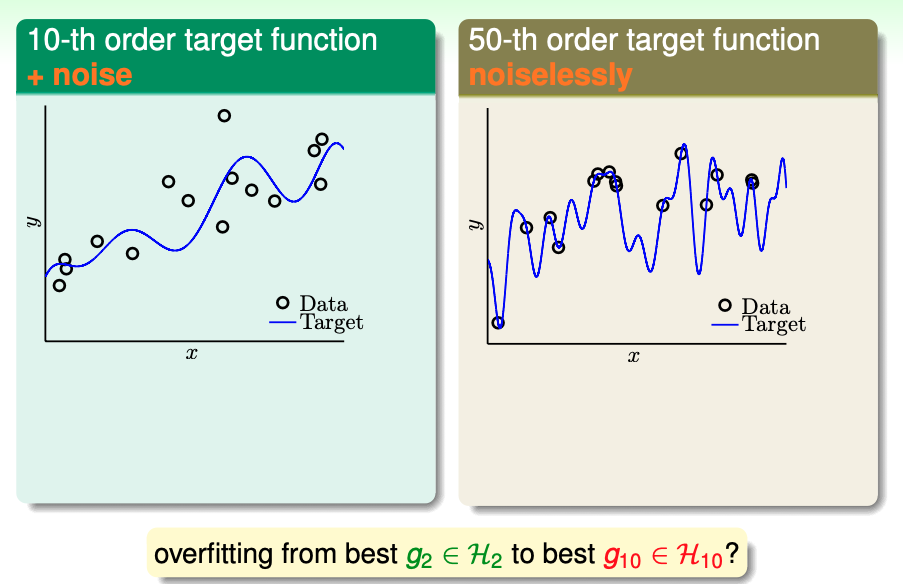
\includegraphics{figure/pdf/overfitting1.png}
  \end{center}
\end{frame}


\begin{frame}{overfitting}
  \begin{center}
    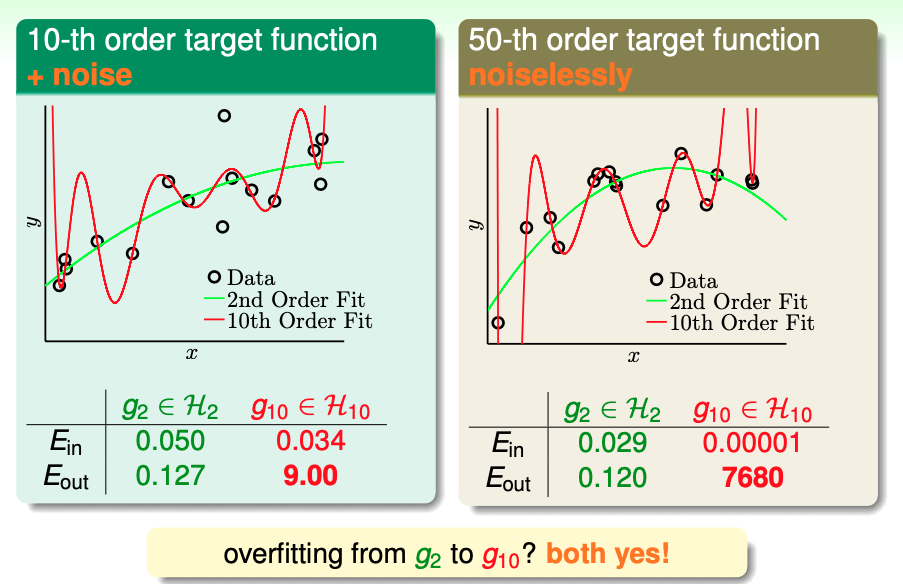
\includegraphics{figure/pdf/overfitting2.png}
  \end{center}
\end{frame}


\begin{frame}{overfitting}
  how to combat overfitting? 
  \begin{itemize}
    \item validation: leave one out, cross validation
    \item early stop
    \item blending (mix multiple model)
  \end{itemize}
\end{frame}


\begin{frame}{elastic net}
  elastic net = weighted lasso and Ridge
  $$
  \min_{\beta} Q(\beta) + \lambda(\alpha||\beta||_2 + (1-\alpha)||\beta||_1)
  $$
  where 
  \begin{itemize}
    \item $Q$: objective function (loss)
    \item $\lambda$: penalty term 
    \item $\alpha$: ratio of mixture
  \end{itemize}

 \vspace{0.5cm} 
  in this paper, thu author build a complex model by including all the features,
  their four-way interactions, and all of the interactions with the quadratic, cubic, and quartic terms of the age variable.
\end{frame}


\begin{frame}{elastic net}
  \begin{center}
    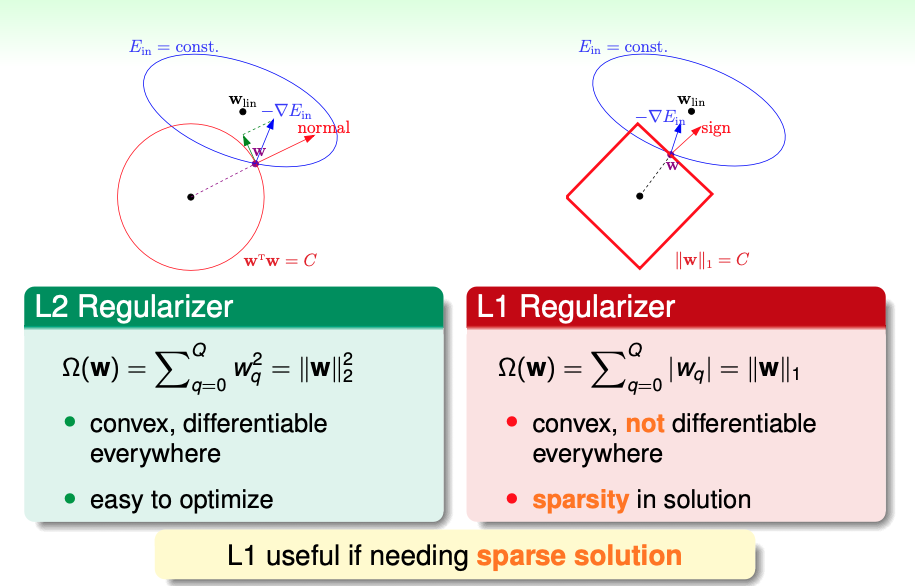
\includegraphics{figure/pdf/regularizer.png}
  \end{center}
\end{frame}


\begin{frame}{Adaptive Boosting}
\begin{center}
  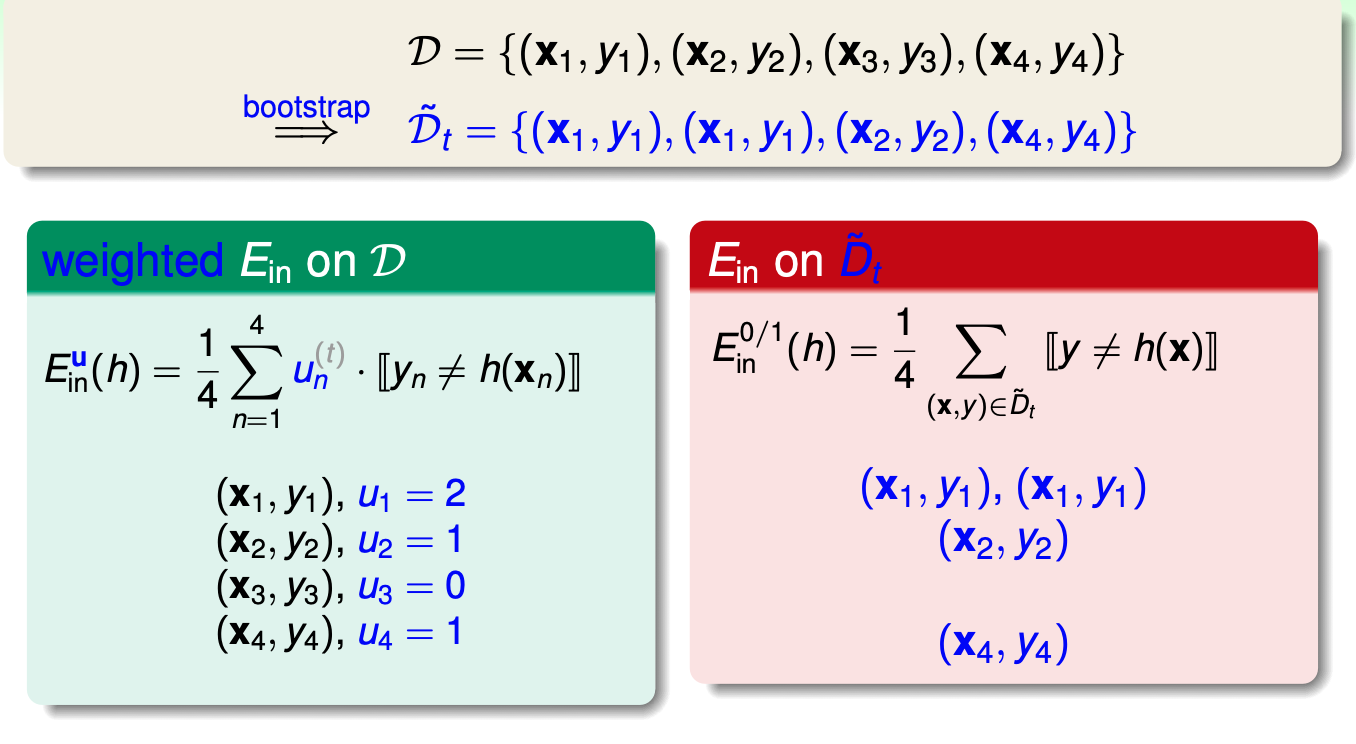
\includegraphics{figure/pdf/boost1.png}
\end{center}
\end{frame}


\begin{frame}{Adaptive Boosting}
\begin{center}
  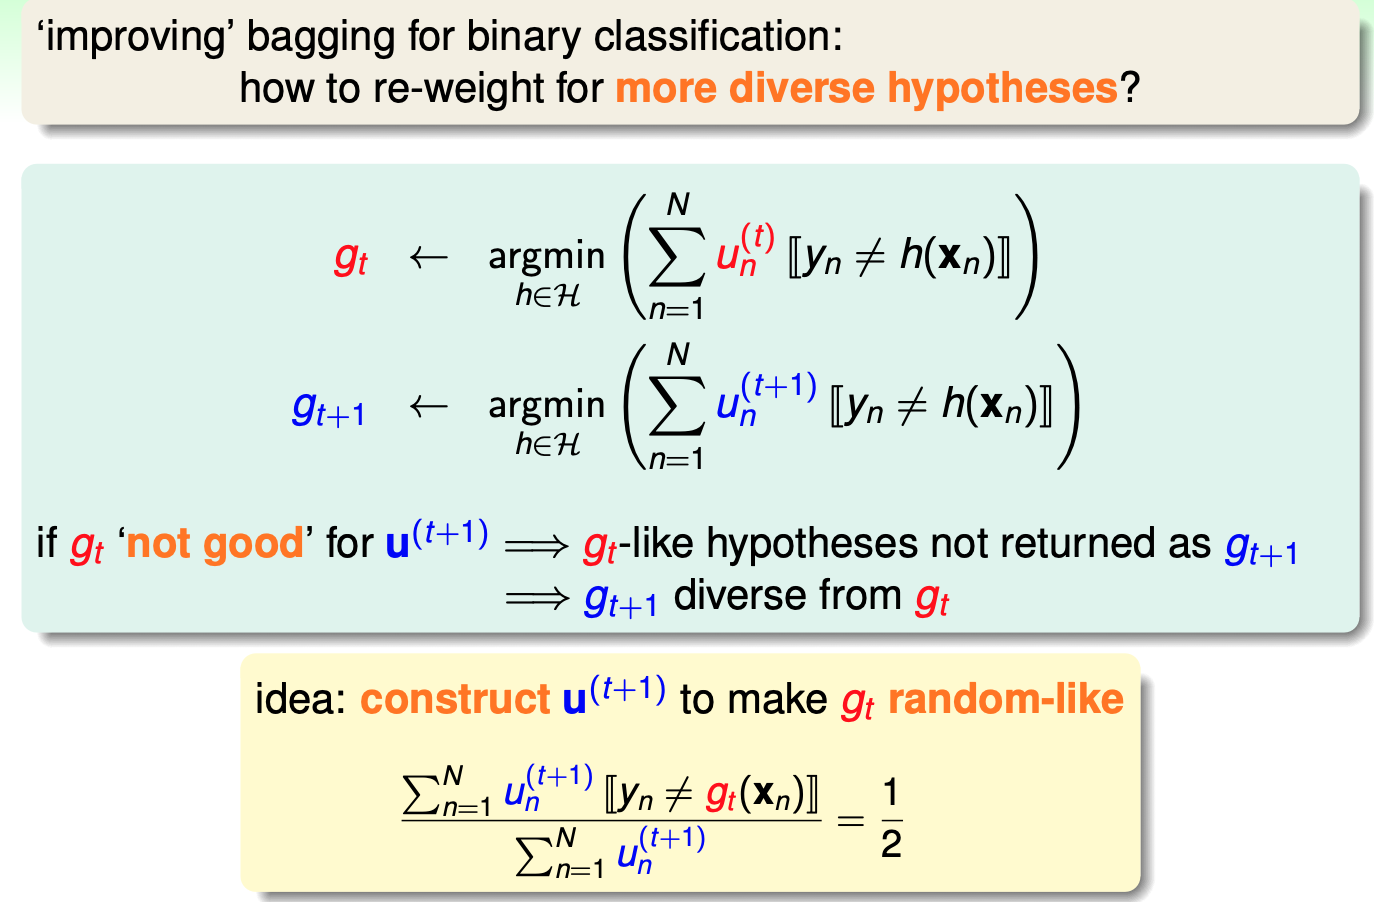
\includegraphics{figure/pdf/boost2.png}
\end{center}
\end{frame}


\begin{frame}{Adaptive Boosting}
$$
\Sigma_{n=1}^N \textcolor{green}{u_n^{t+1}}\mathbbm{1}(y_n = g_t(x_n)) = \Sigma_{n=1}^N \textcolor{red}{u_n^{t+1}}\mathbbm{1}(y_n \neq g_t(x_n))
$$
\begin{multline*}
  \Sigma_{n=1}^N \textcolor{green}{\Sigma_{n=1}^N u_n^{t+1}\mathbbm{1}(y_n \neq g_t(x_n))} \mathbbm{1}(y_n = g_t(x_n)) =  \\
  \Sigma_{n=1}^N \textcolor{red}{\Sigma_{n=1}^N u_n^{t+1}\mathbbm{1}(y_n = g_t(x_n))} \mathbbm{1}(y_n \neq g_t(x_n))
\end{multline*}

\begin{multline*}
  \Sigma_{n=1}^N \textcolor{green}{\frac{\Sigma_{n=1}^N u_n^{t+1}\mathbbm{1}(y_n \neq g_t(x_n))}{\Sigma_{n=1}^N u_n^{t+1}}} \mathbbm{1}(y_n = g_t(x_n)) =  \\
  \Sigma_{n=1}^N  \textcolor{red}{\frac{\Sigma_{n=1}^N u_n^{t+1}\mathbbm{1}(y_n = g_t(x_n))}{\Sigma_{n=1}^N u_n^{t+1}}} \mathbbm{1}(y_n \neq g_t(x_n))
\end{multline*}
\end{frame}


\begin{frame}{Adaptive Boosting}
$$
  \Sigma_{n=1}^N \textcolor{green}{\epsilon_{t+1}} \mathbbm{1}(y_n = g_t(x_n)) =
  \Sigma_{n=1}^N \textcolor{red}{(1-\epsilon_{t+1})} \mathbbm{1}(y_n \neq g_t(x_n))
$$
$$
  \Sigma_{n=1}^N \textcolor{green}{\sqrt{\epsilon_{t+1}^2}} \mathbbm{1}(y_n = g_t(x_n)) =
  \Sigma_{n=1}^N \textcolor{red}{\sqrt{(1-\epsilon_{t+1})^2}} \mathbbm{1}(y_n \neq g_t(x_n))
$$
$$
  \Sigma_{n=1}^N \textcolor{green}{\sqrt{\frac{\epsilon_{t+1}^2}{\epsilon_{t+1}(1-\epsilon_{t+1})}}} \mathbbm{1}(y_n = g_t(x_n)) =
 \Sigma_{n=1}^N  \textcolor{red}{\sqrt{\frac{(1-\epsilon_{t+1})^2}{\epsilon_{t+1}(1-\epsilon_{t+1})}}} \mathbbm{1}(y_n \neq g_t(x_n))
$$
$$
  \Sigma_{n=1}^N \textcolor{green}{\sqrt{\frac{\epsilon_{t+1}}{(1-\epsilon_{t+1})}}} \mathbbm{1}(y_n = g_t(x_n)) =
  \Sigma_{n=1}^N \textcolor{red}{\sqrt{\frac{(1-\epsilon_{t+1})}{\epsilon_{t+1}}}} \mathbbm{1}(y_n \neq g_t(x_n))
$$
$$
\Sigma_{n=1}^N \textcolor{green}{\frac{1}{\blacklozenge_{t+1}}}  \mathbbm{1}(y_n = g_t(x_n))  =
\Sigma_{n=1}^N \textcolor{red}{\blacklozenge_{t+1}}  \mathbbm{1}(y_n \neq g_t(x_n)) 
$$
$$
\begin{cases}
  \blacklozenge_{t+1} >= 1 & \iff \epsilon_{t+1} <= \frac{1}{2} \\
  \alpha_{t+1} = \log(\blacklozenge_{t+1}) >= 0 & \iff \blacklozenge_{t+1} >= 1
\end{cases}
$$
\end{frame}


\begin{frame}{Adaptive Boosting}
\begin{center}
  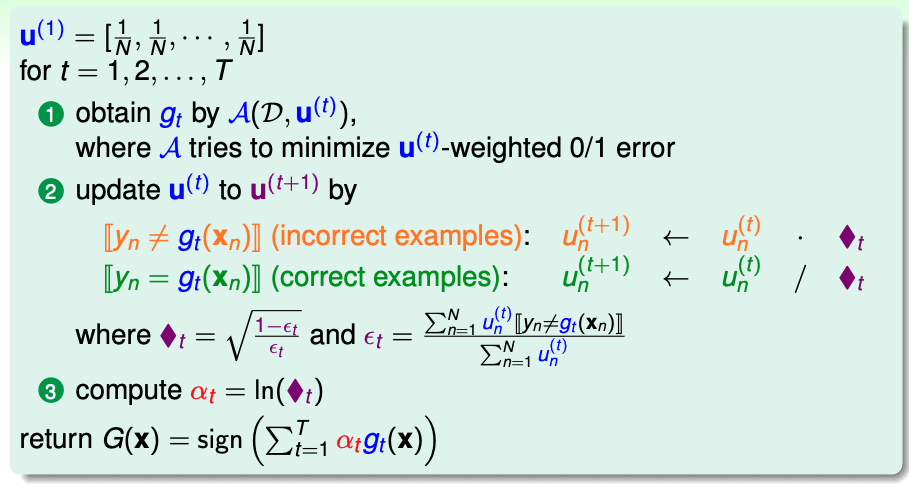
\includegraphics{figure/pdf/boost3.png}
\end{center}
\end{frame}


\begin{frame}{Adaptive Boosting}
  \href{https://github.com/githubjacky/HTML/blob/main/hw5/utils.jl}{Julia implementation}
  \begin{center}
    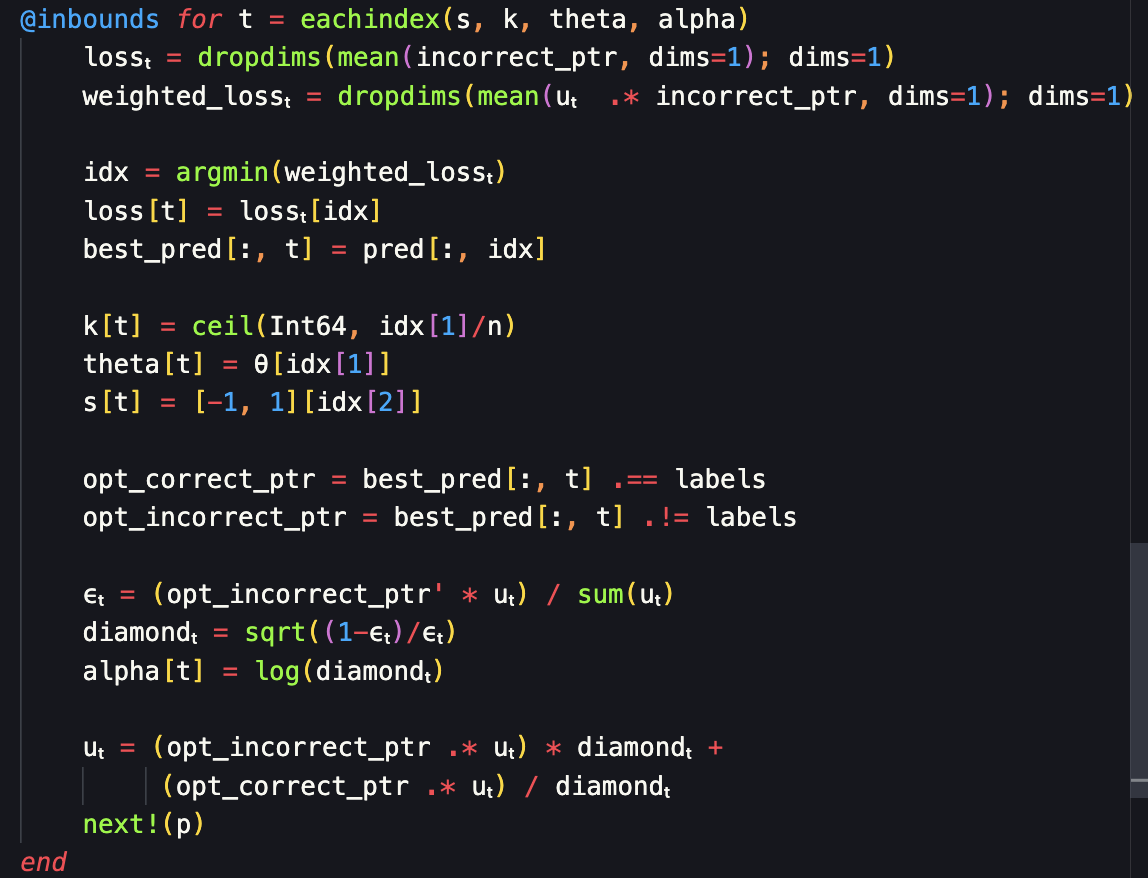
\includegraphics[width=0.7\textwidth]{figure/pdf/adaboost.png}
  \end{center}
\end{frame}


\begin{frame}{Gradient Boosting}
  \begin{center}
    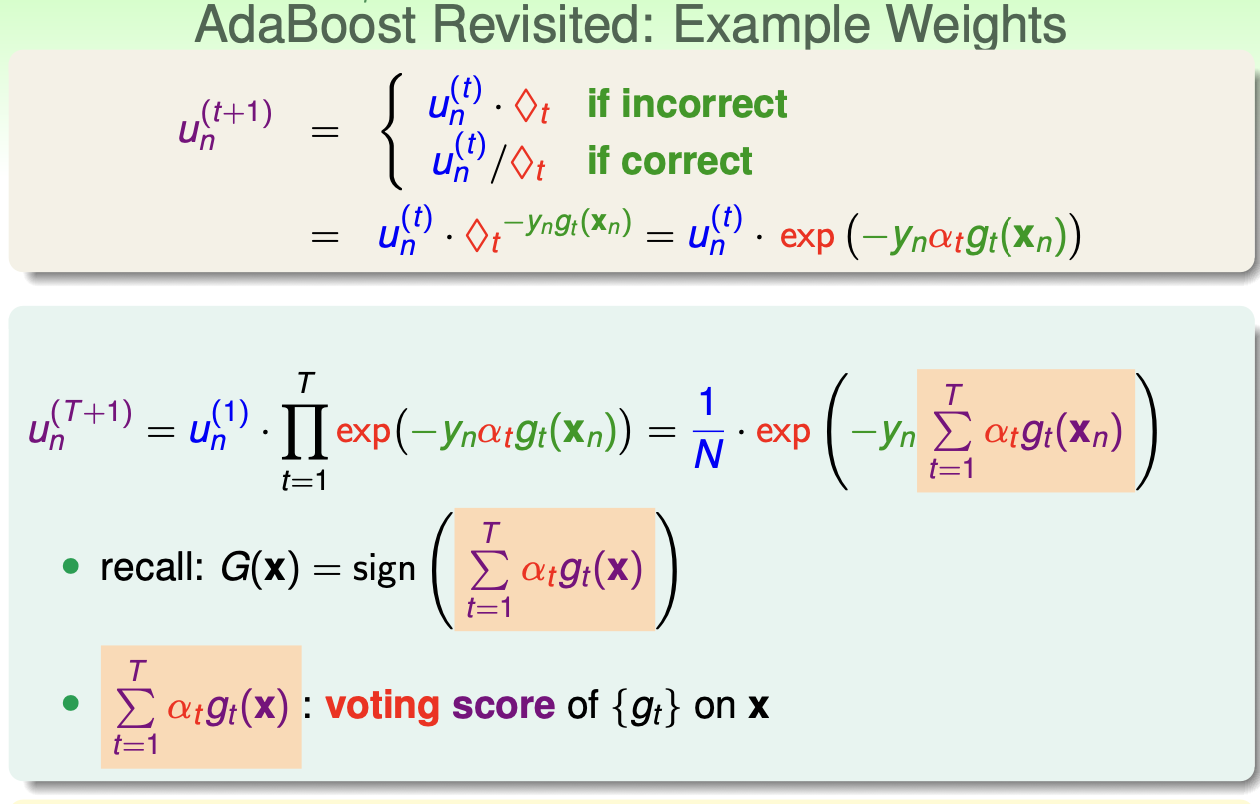
\includegraphics[width=0.9\textwidth]{figure/pdf/gbm.png}
  \end{center}
\end{frame}


\begin{frame}{SVM}
  \begin{center}
    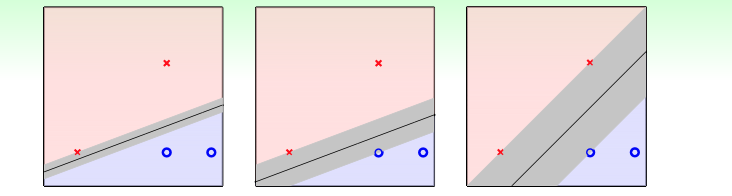
\includegraphics{figure/pdf/svm1.png}
  \end{center}
  \begin{center}
    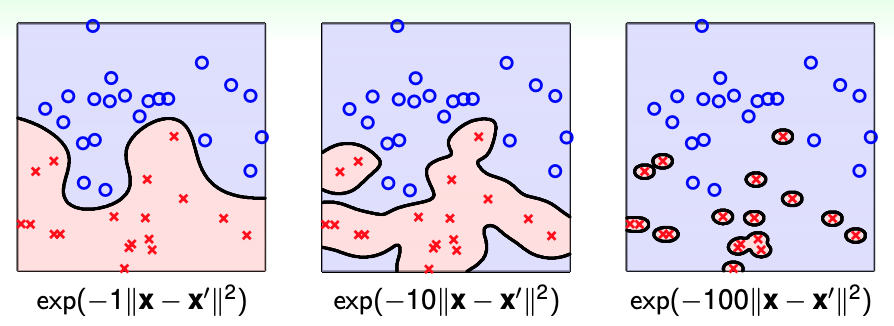
\includegraphics{figure/pdf/svm2.png}
  \end{center}
\end{frame}

\begin{frame}{methodology}
\begin{itemize}
  \item use the machine learning model to predict who might be a potential minimum wage worker
  \begin{itemize}
    \item hourly wage of less than 125\% of the statutory minimum wage
    \item high probability group: comprises the 10\% of the population with the hightest 
          likelihood of being affected by the policy.
    \item high recall group: 75\% of all minimum wage workers are captured
  \end{itemize}
  \item worker-level selection criterion
  \begin{itemize}
    \item there had not had been any prominent minimum wage events in the past 20 quarters
    \item there is a prominent minimum wage change in the next 12 quarters
    \item 469,174 observations, randomly draw 150, 000 for training
  \end{itemize}
\end{itemize}
\end{frame}


\begin{frame}{methodology}
\begin{itemize}
  \item prominent minimum wage change
  \begin{itemize}
    \item (real)minimum wages increased by more than \$0.25
    \item at least 2\% of the workforce earned between the new minimum wage and the old minimum wage
  \end{itemize}
  \item use DID to esitmate the change of wage, employment, unemployment, LFP in two groups
  \begin{itemize}
    \item 8-year window around 172 prominent state-level minimum wage events
    \item $y_{st}^g = \Sigma_{\tau=-3}^4 \beta_{\tau}treat_{st}^{\tau} + \Omega_{st} + \mu_s + \rho_t + u_{st}$
    \item $\Omega_{st}$: for small or federal in-creases (Cengiz et al. (2019))
    \item $treat_{st}^{\tau}$: whether the minimum wage was increased $\tau$ years from date t in state s
    \item cluster standard error by states
  \end{itemize}
\end{itemize}
  
\end{frame}


\begin{frame}{confusion matrix}
\begin{center}
  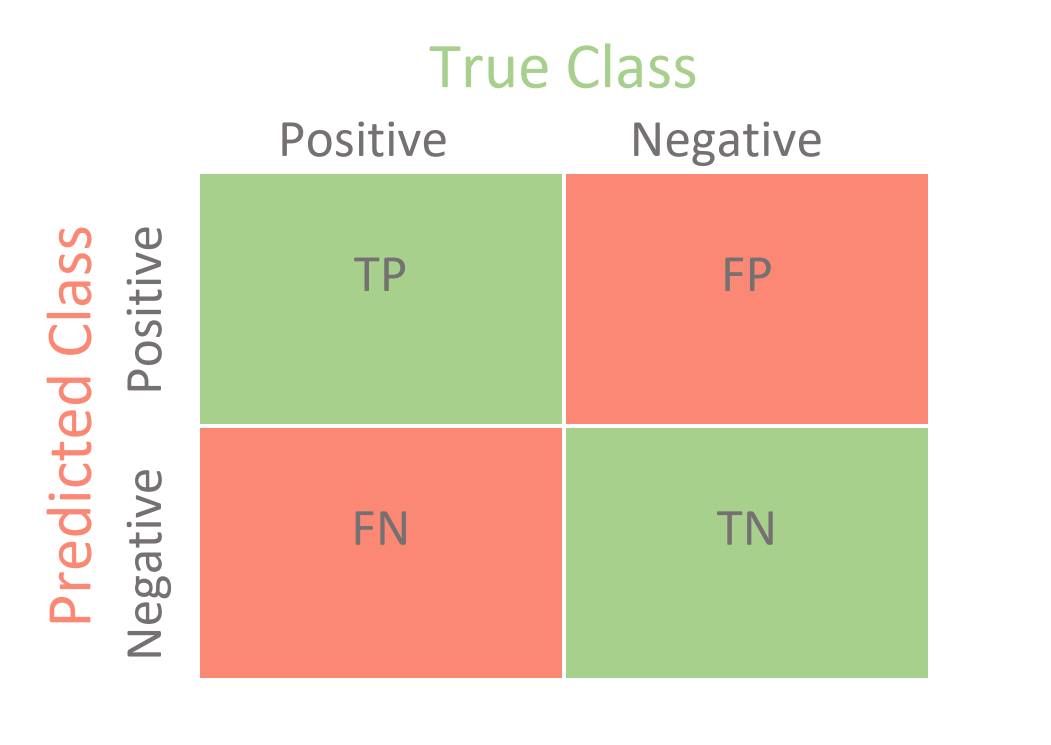
\includegraphics{figure/pdf/confustion_matrix.png}
\end{center}
\end{frame}


\begin{frame}{confusion matrix}
  \begin{itemize}
    \item Accuracy: $\frac{TP+TN}{TP+FN+FP+TN}$
    \item precision: $\frac{TP}{TP+FP}$
    \item recall(sensitivity, true positive rate): $\frac{TP}{TP+FN}$
    \item false positive rate: $\frac{FP}{FP+TN}$
  \end{itemize}
\end{frame}


\begin{frame}{ROC AUC}
  \begin{center}
    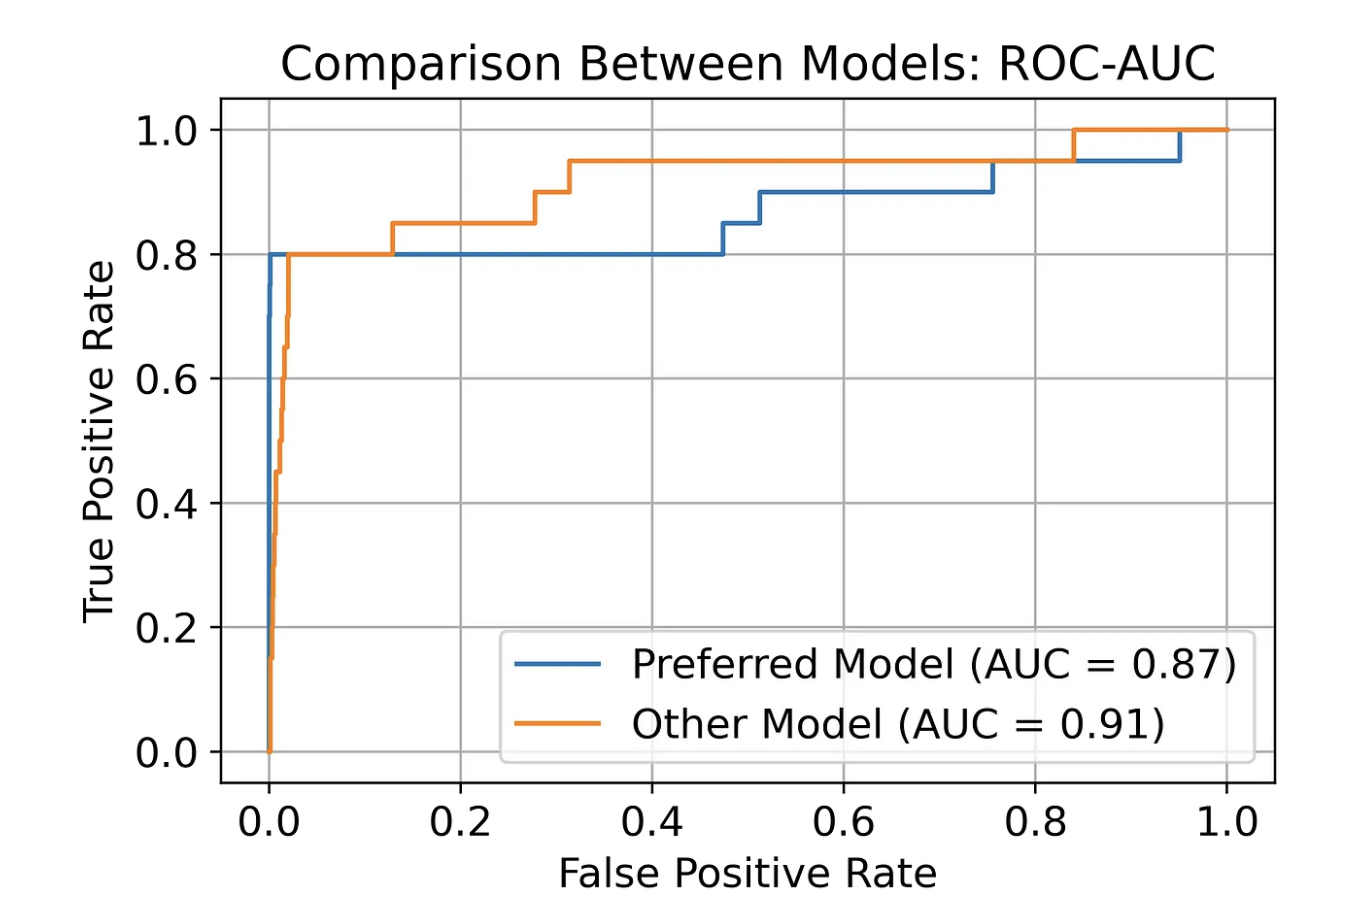
\includegraphics{figure/pdf/roc_auc.png}
  \end{center}
\end{frame}


\begin{frame}{AUPRC}
  \begin{center}
    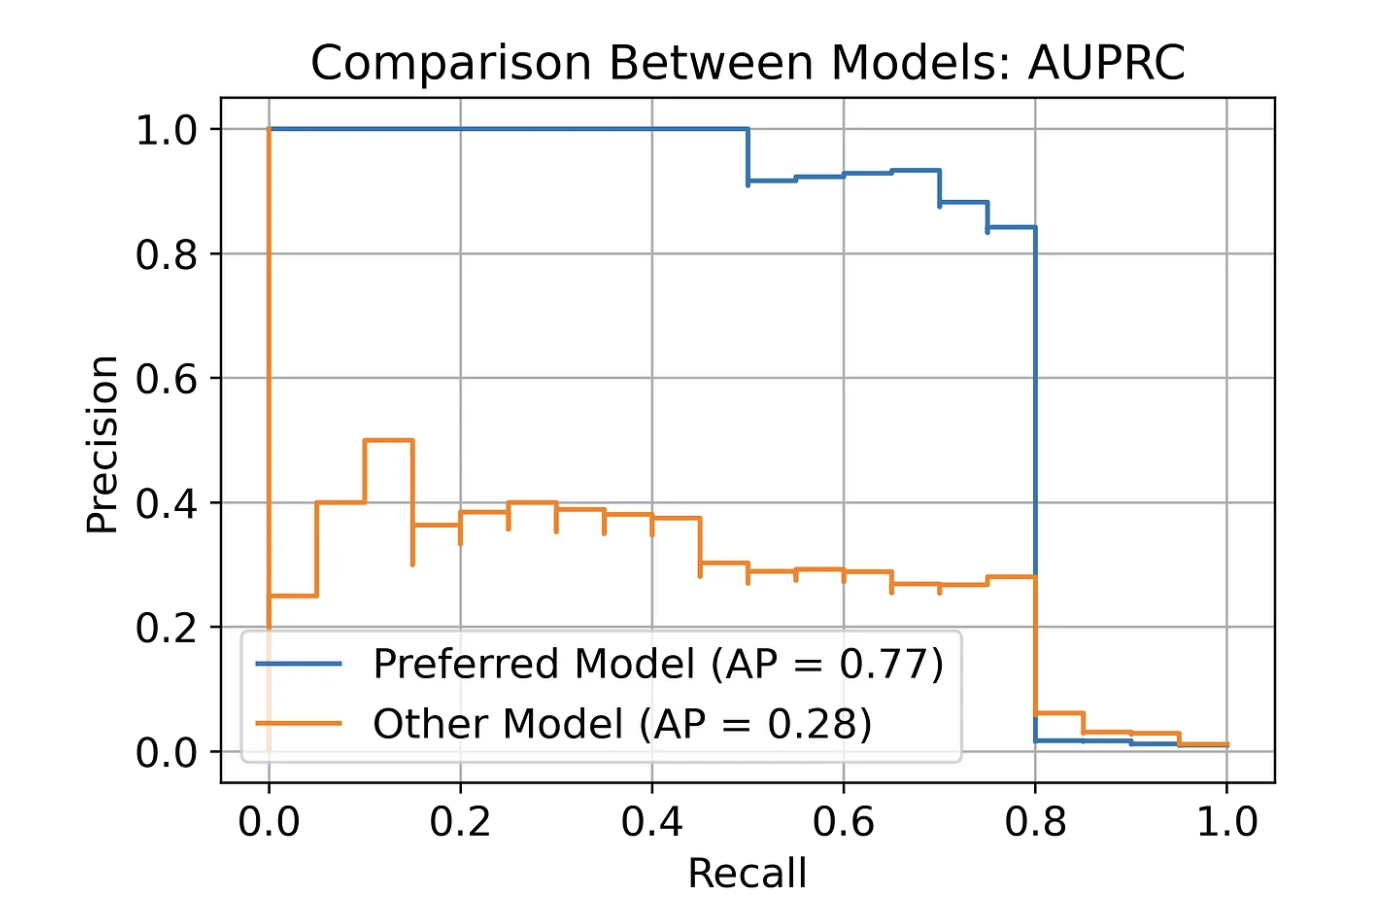
\includegraphics{figure/pdf/auprc.png}
  \end{center}
\end{frame}


\begin{frame}{data and features}
  \begin{itemize}
    \item minimum wage worker prediciton: 1979-2019 CPS-ORG
    \begin{itemize}
      \item Education group
      \item Age group
      \item Gender
      \item Rural residency
      \item Martial(married and spouse is present)
      \item Race 
      \item Hispanic
      \item Veteran
    \end{itemize}
    \item labor market outcomes estimation: 1979-2019 CPS-Basic
  \end{itemize}
\end{frame}


\begin{frame}{evaluation}
  \begin{center}
    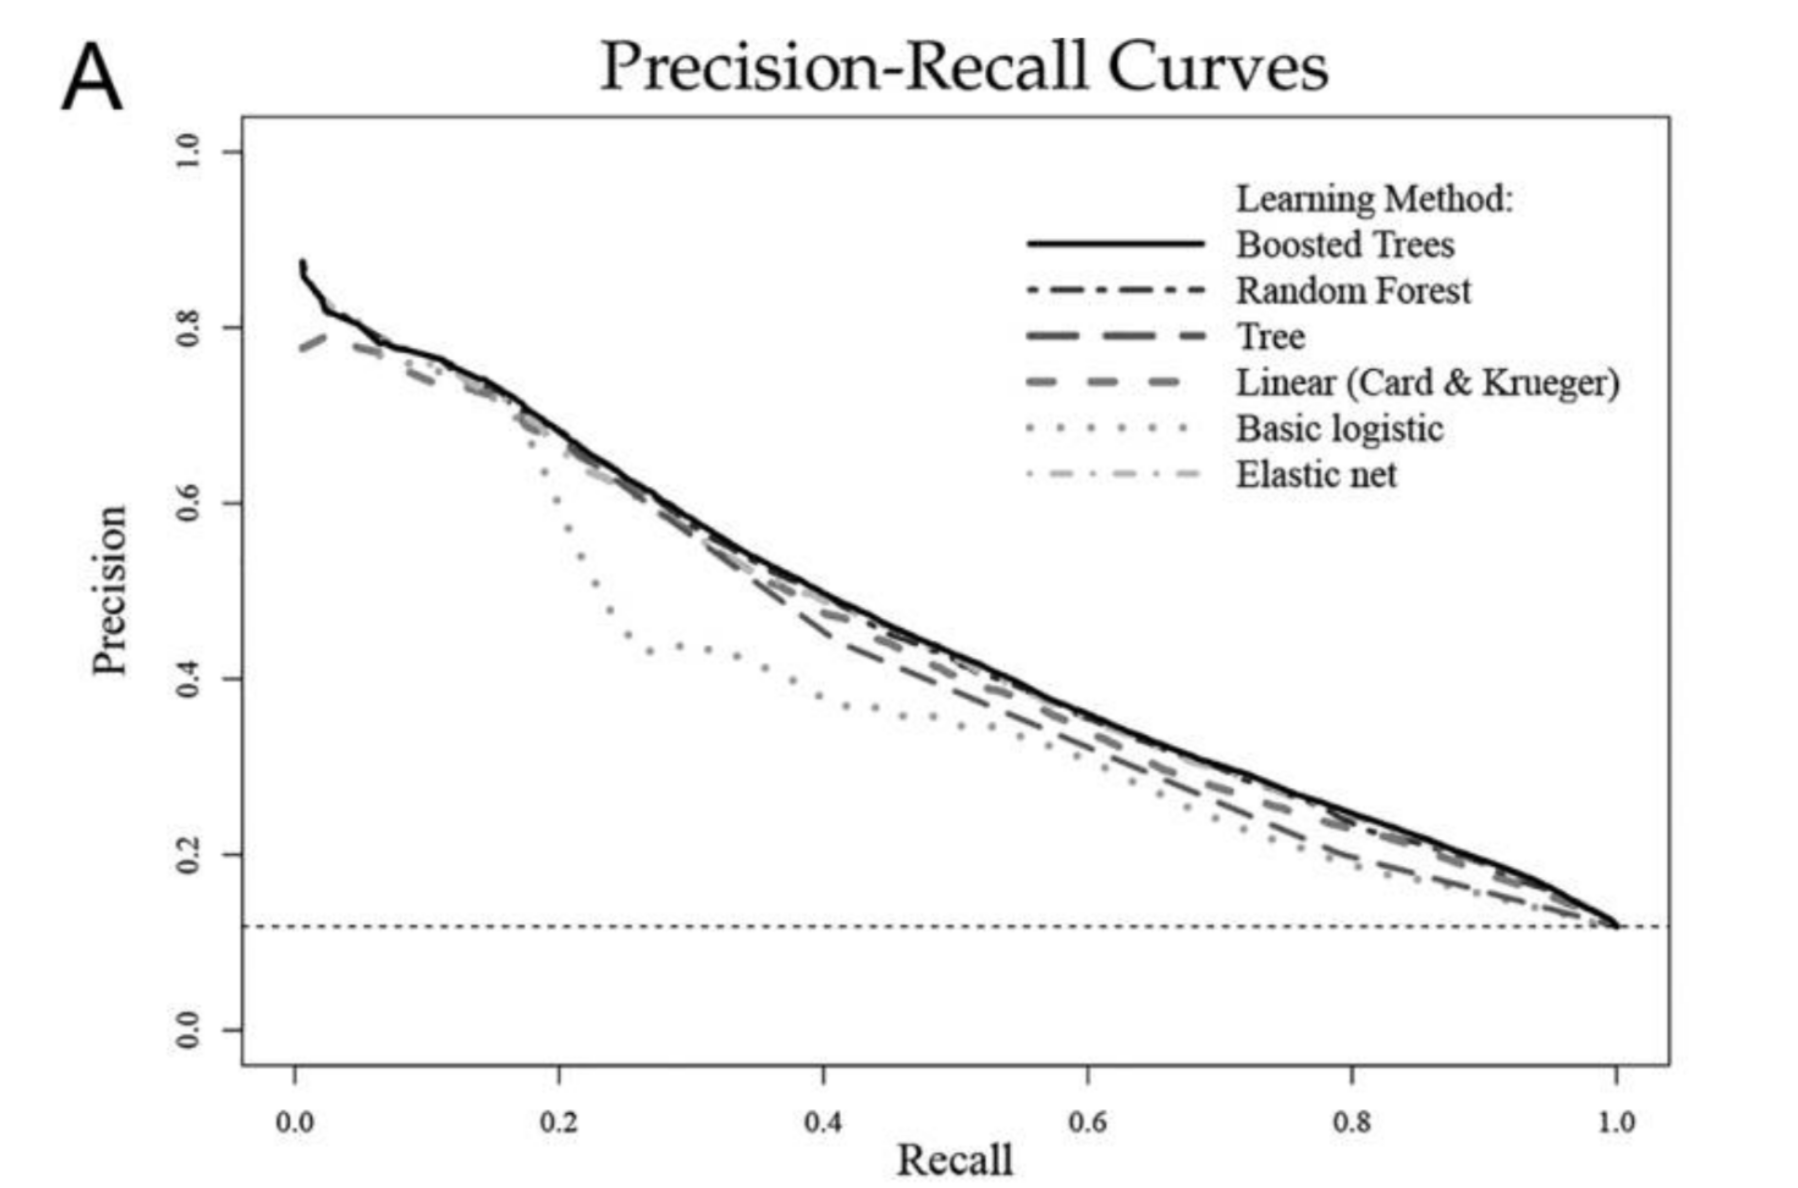
\includegraphics{figure/pdf/evaluation.png}
  \end{center}
\end{frame}


\begin{frame}{evaluation}
  \begin{itemize}
    \item high probability group
    \begin{itemize}
      \item threshold probability 0.35
      \item precision: 0.6
      \item recall: 0.36
    \end{itemize}
    \item high recall group
    \begin{itemize}
      \item threshold probability 0.12
      \item precision: 0.35
      \item recall: 0.75
    \end{itemize}
    \item low probability group: predicted probability $\le$ 0.12
  \end{itemize}
\end{frame}


\begin{frame}{who is a minimum wage worker}
  \begin{center}
    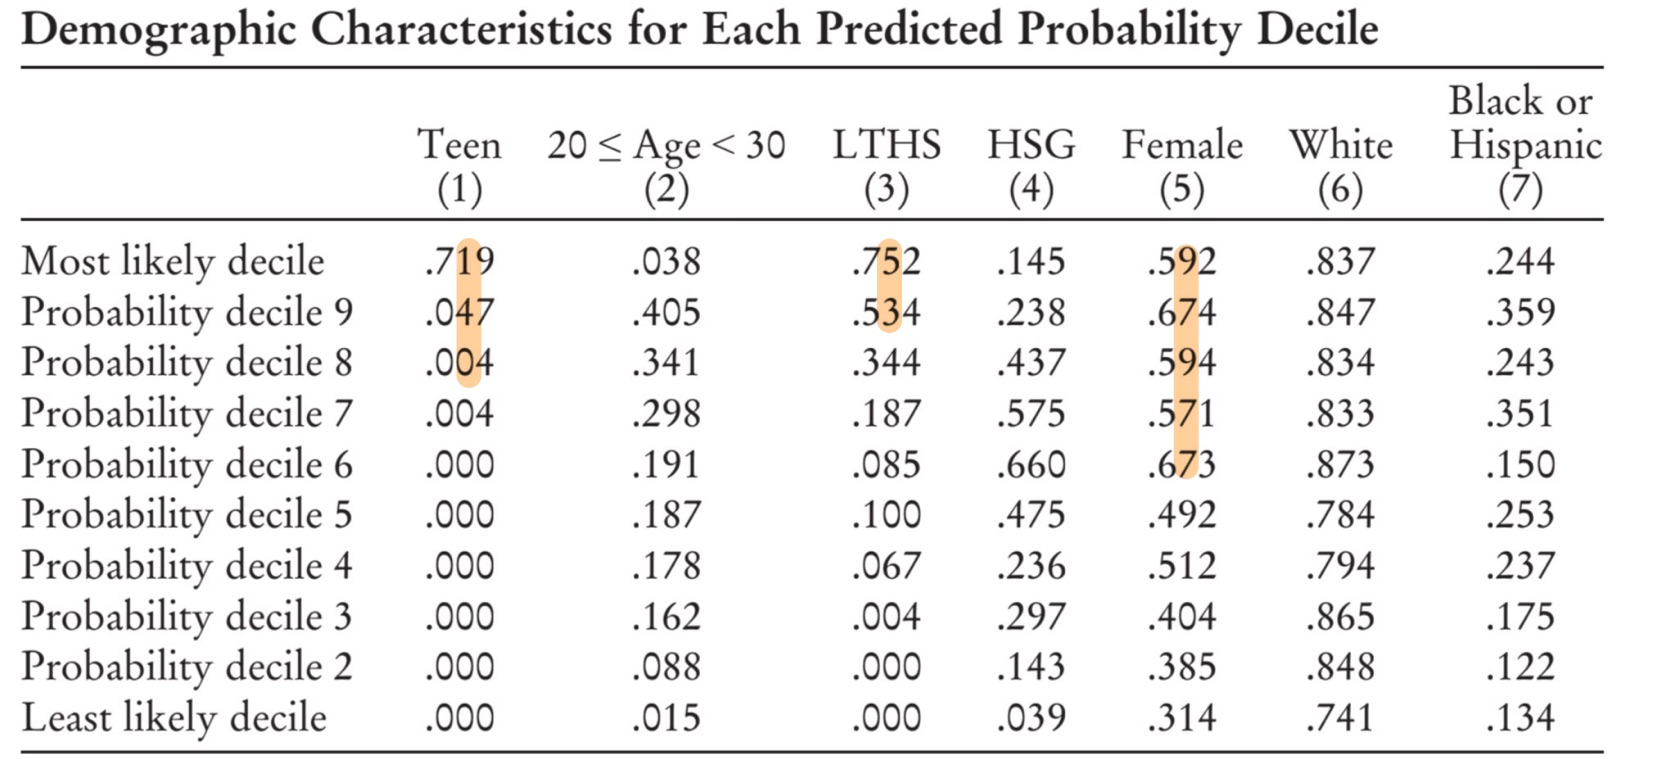
\includegraphics{figure/pdf/decitle.jpg}
  \end{center}
\end{frame}


\begin{frame}{who is a minimum wage worker}
  \begin{center}
    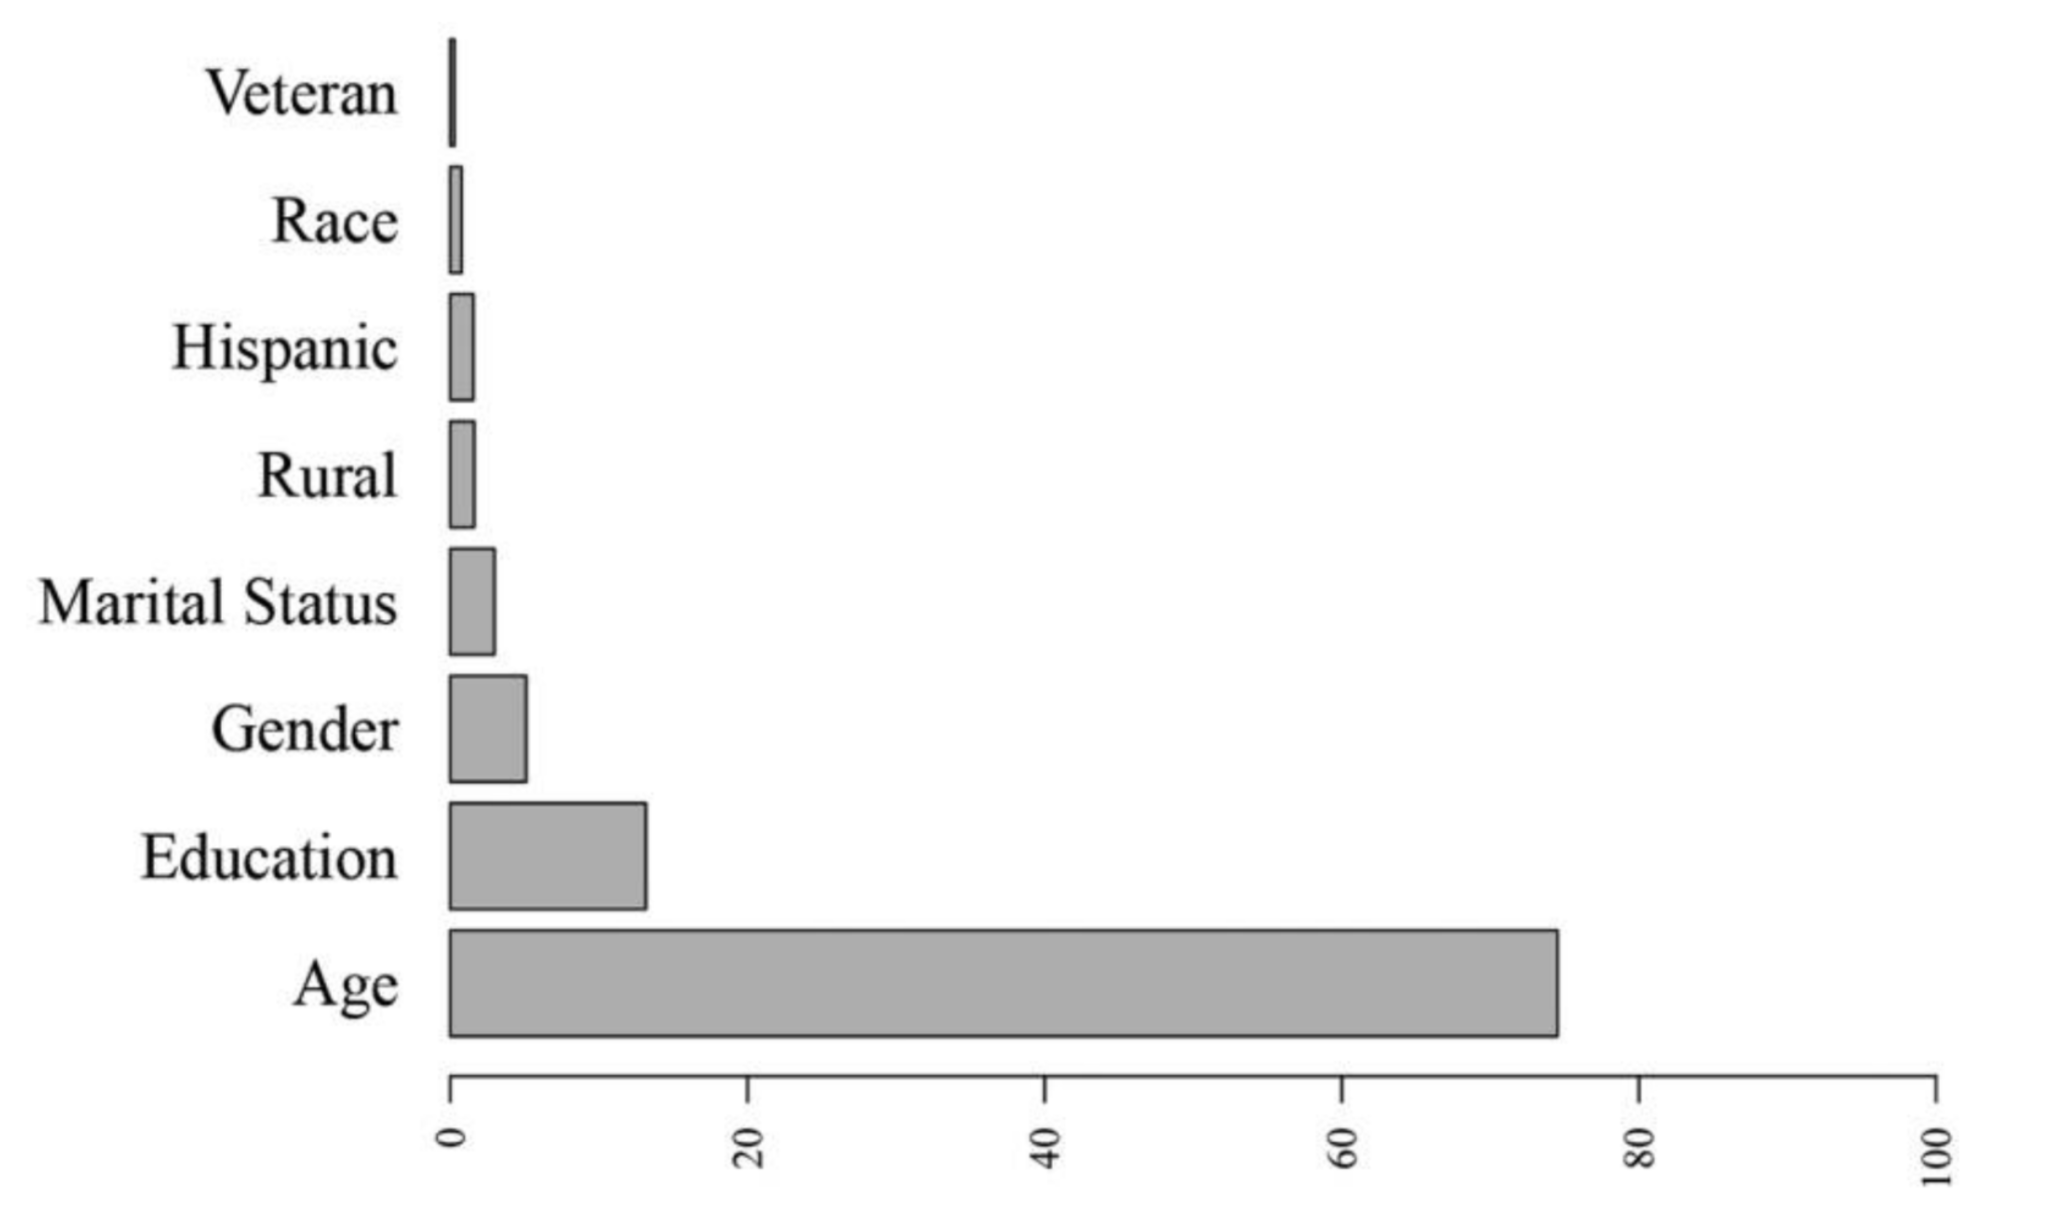
\includegraphics{figure/pdf/tree_importance.png}
  \end{center}
\end{frame}

\begin{frame}{labor market outcome}
  \begin{itemize}
    \item 5-year averaged posttreatment estimates: $\frac{1}{5} \Sigma_{\tau=0}^4(\beta_{\tau} - \beta_{-1})$
    \item wage
    \begin{itemize}
      \item high probability: 2.3\%(SE, 0.3\%)
      \item high recall: 1.6\% (SE, 0.3\%)
      \item low probability: -0.1\% (SE, 0.3\%)
    \end{itemize}
  \end{itemize}
\end{frame}

\begin{frame}{high probability estimation}
  \begin{center}
    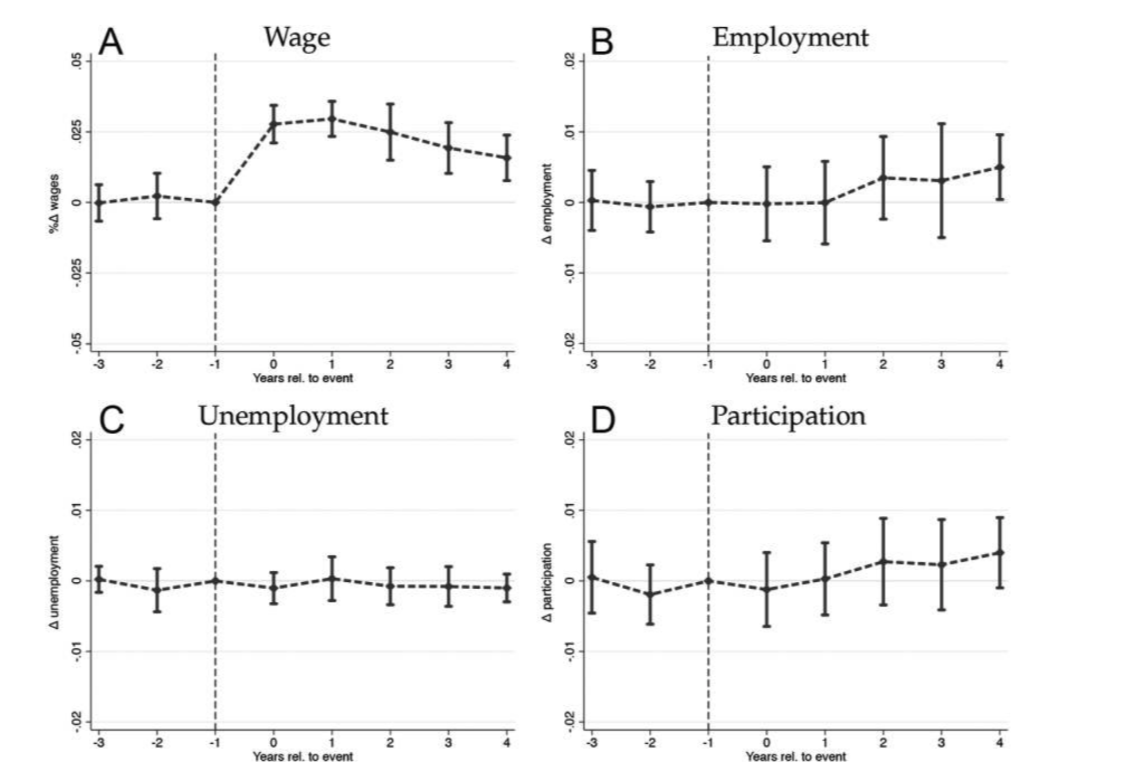
\includegraphics{figure/pdf/high_proba_res.png}
  \end{center}
\end{frame}

\begin{frame}{high recall estimation}
  \begin{center}
    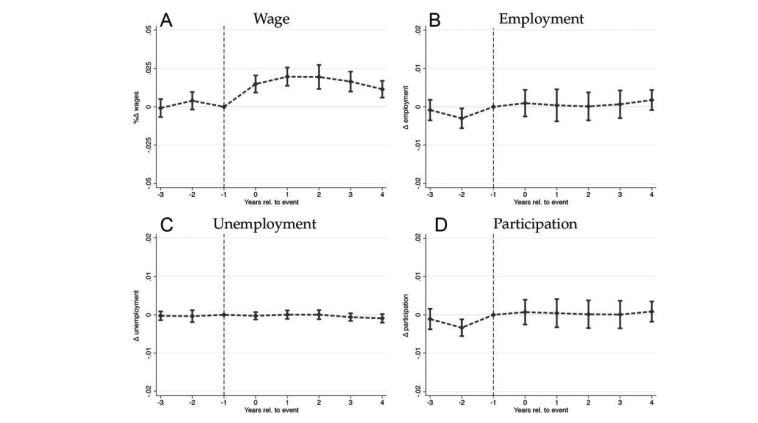
\includegraphics{figure/pdf/high_recall_res.png}
  \end{center}
\end{frame}


\begin{frame}{hands-on machine learning}
  Let's apply the framework using Taiwan's Data
\end{frame}


\begin{frame}{data}
  \begin{itemize}
    \item source: 行政院主計處\ \href{https://srda.sinica.edu.tw/browsingbydatatype_result.php?category=surveymethod&type=4&csid=31}{人力資源運用調查, 2000-2006}
    \item features: countycat, sex, martial, educat, agecat
    \begin{itemize}
      \item martial: married or not
      \item educat
      \begin{itemize}
        \item 1: below junior high
        \item 2: high school
        \item 3: at least college
      \end{itemize}
      \item agecat: group every 5 years from 15 to 70 as one category
    \end{itemize}
  \end{itemize}
\end{frame}


\begin{frame}{tidymodels}
  pipeline for training a machine learning models
  \begin{enumerate}
    \item before training: preprocess and specify the model
    \begin{itemize}
      \item recipes, parsnip
    \end{itemize}
    \item hyperparameters tuning and evaluation
    \begin{itemize}
      \item rsample, tune, yardstick
    \end{itemize}
    \item prediction and evaluation
    \begin{itemize}
      \item yardstick
    \end{itemize}
  \end{enumerate}
\end{frame}


\begin{frame}{data}
  \begin{center}
    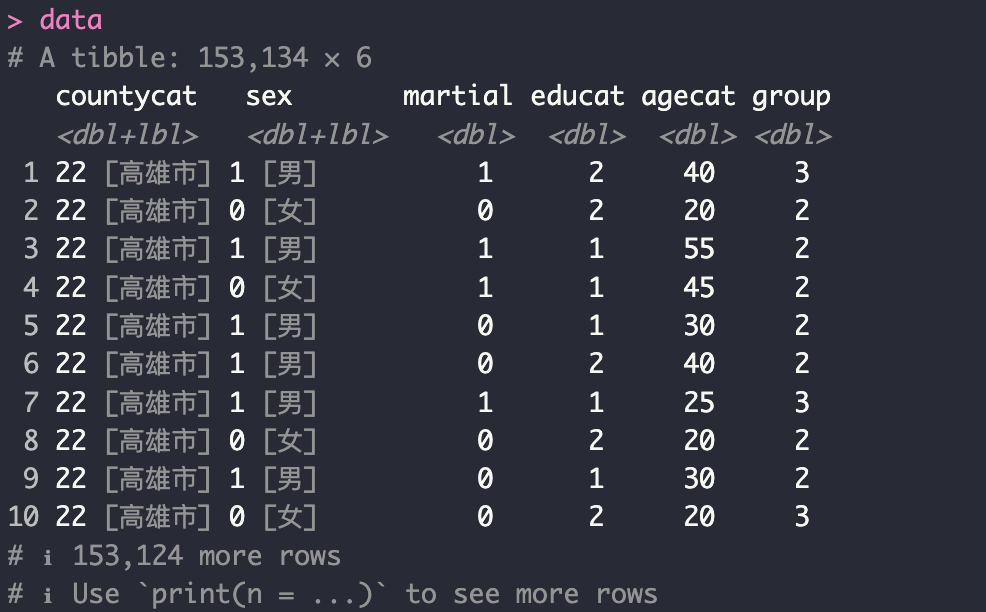
\includegraphics[width=0.8\textwidth]{figure/pdf/code1.png}
  \end{center}
\end{frame}


\begin{frame}{helper function}
  \begin{center}
    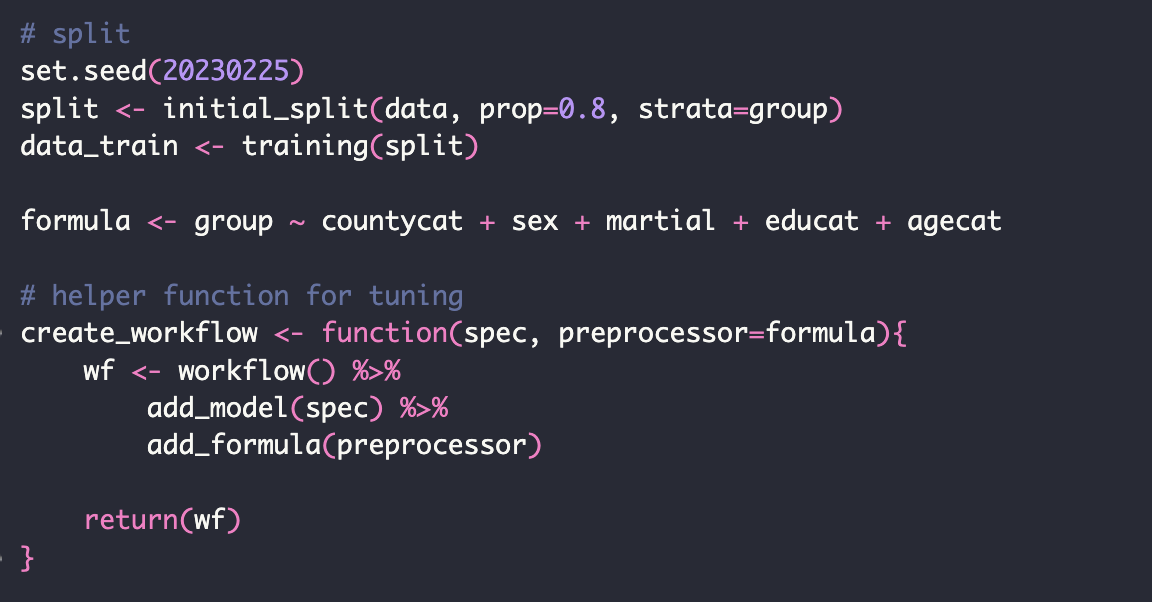
\includegraphics[width=0.9\textwidth]{figure/pdf/code2.png}
  \end{center}
\end{frame}


\begin{frame}{helper function}
  \begin{center}
    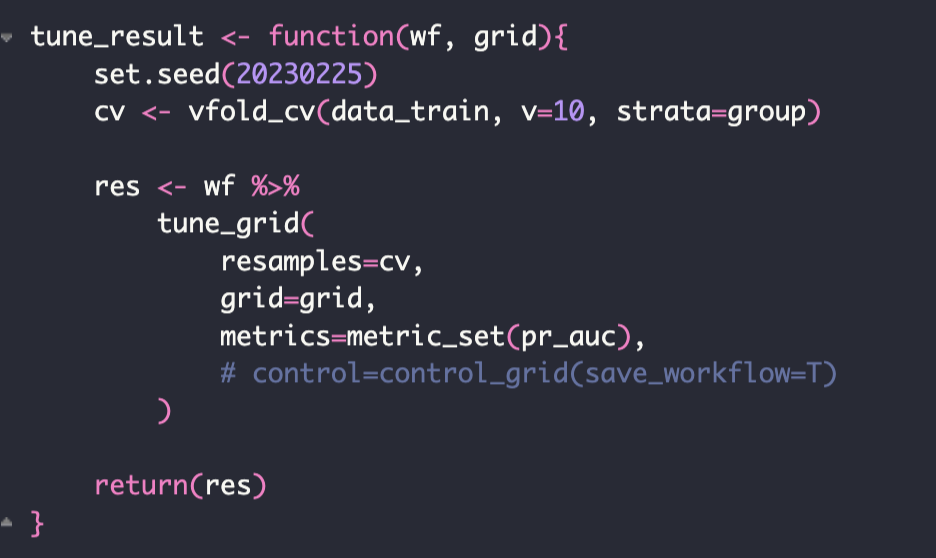
\includegraphics[width=0.9\textwidth]{figure/pdf/code3.png}
  \end{center}
\end{frame}


\begin{frame}{helper function}
  \begin{center}
    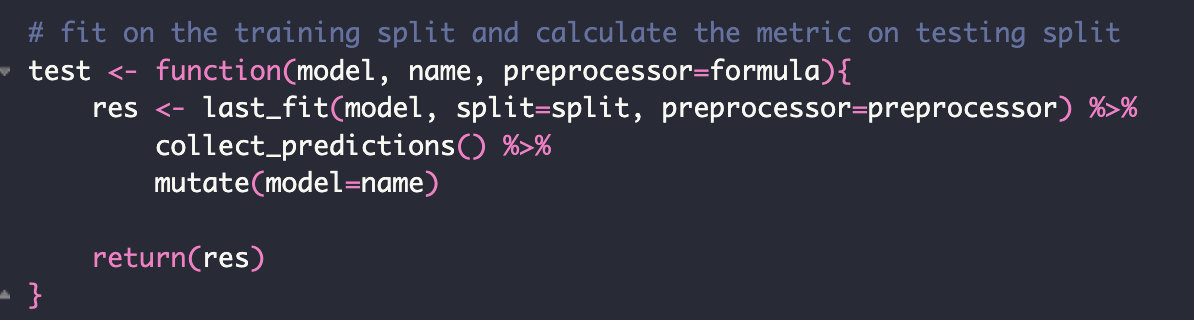
\includegraphics{figure/pdf/code4.png}
  \end{center}
\end{frame}


\begin{frame}{elastic net}
  \begin{center}
    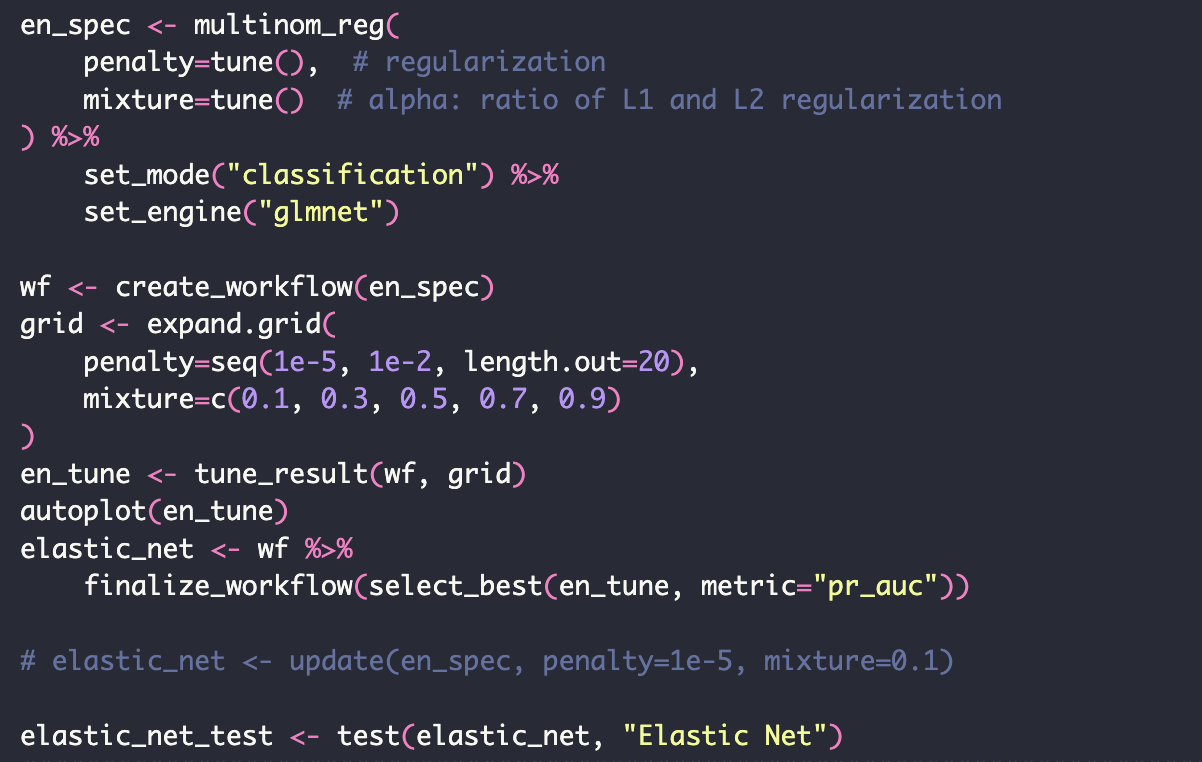
\includegraphics{figure/pdf/en.png}
  \end{center}
\end{frame}


\begin{frame}{elastic net}
  \begin{center}
    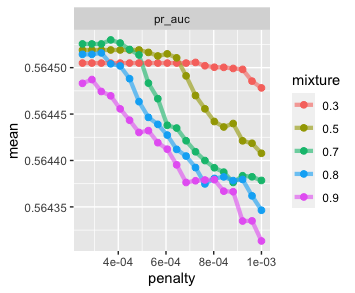
\includegraphics[width=0.8\textwidth]{figure/pdf/en_tune.png}
  \end{center}
\end{frame}


\begin{frame}{random forest}
  \begin{center}
    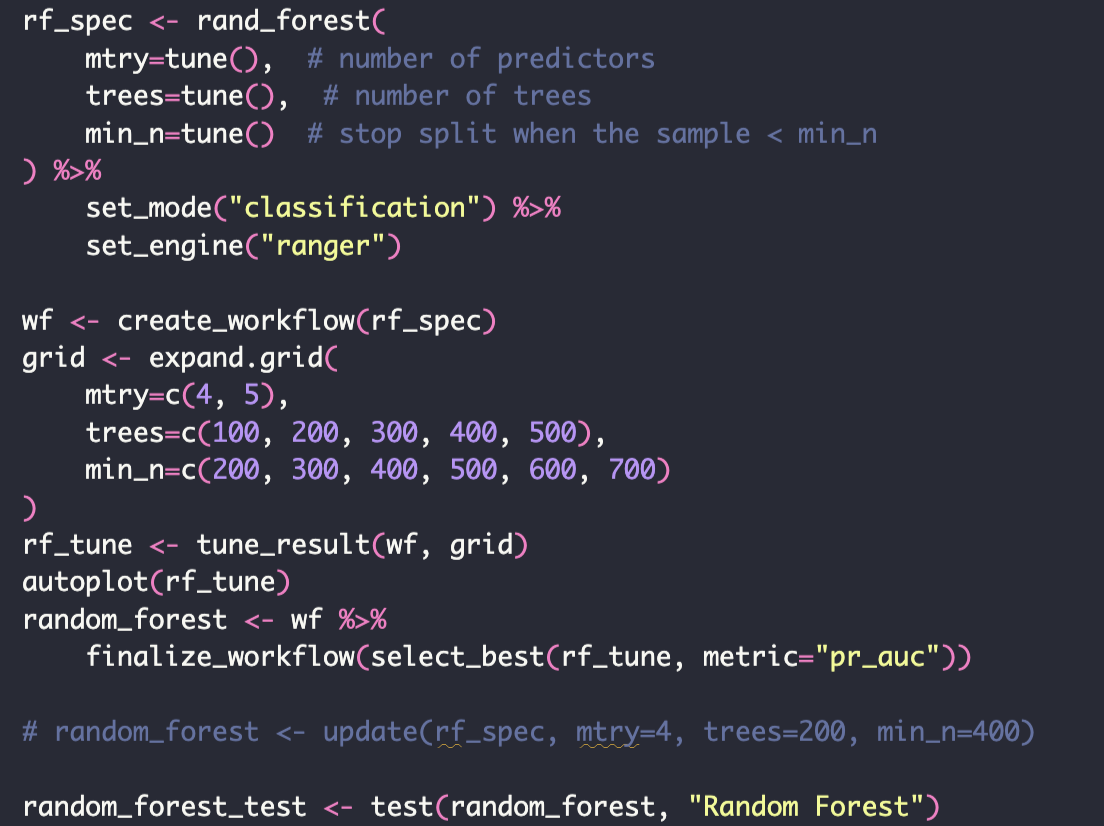
\includegraphics[width=0.9\textwidth]{figure/pdf/rf.png}
  \end{center}
\end{frame}


\begin{frame}{random forest}
  \begin{center}
    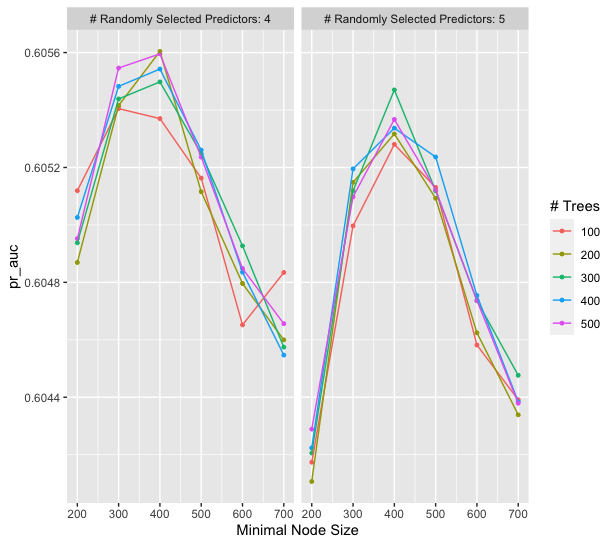
\includegraphics[width=0.7\textwidth]{figure/pdf/rf_tune.png}
  \end{center}
\end{frame}


\begin{frame}{XGBoost}
  \begin{center}
    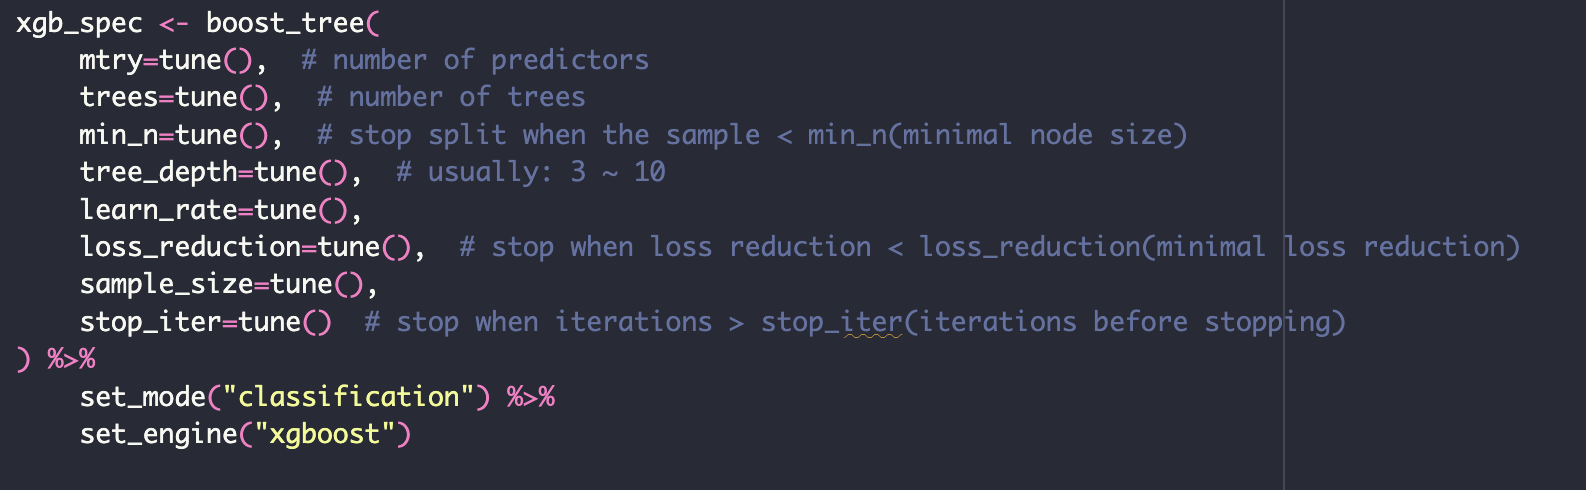
\includegraphics{figure/pdf/xgb1.png}
  \end{center}
\end{frame}


\begin{frame}{XGBoost}
  \begin{itemize}
    \item tuning strategy
    \begin{enumerate}
      \item tune min\_n, tree\_depth
      \item default suggestion
      \begin{itemize}
        \item mtry: 80\%of the predictors
        \item trees: 200
        \item loss\_reduction = 0
        \item sample\_size: 80\% of the sample size
        \item stop\_iter = 2000(should be large enough)
      \end{itemize}
      \item tune mtry, sample\_size
      \item tune trees, loss\_reduction, stop\_iter
      \item tune the learn\_rate
    \end{enumerate}
  \end{itemize}
\end{frame}


\begin{frame}{XGBoost}
  \begin{center}
    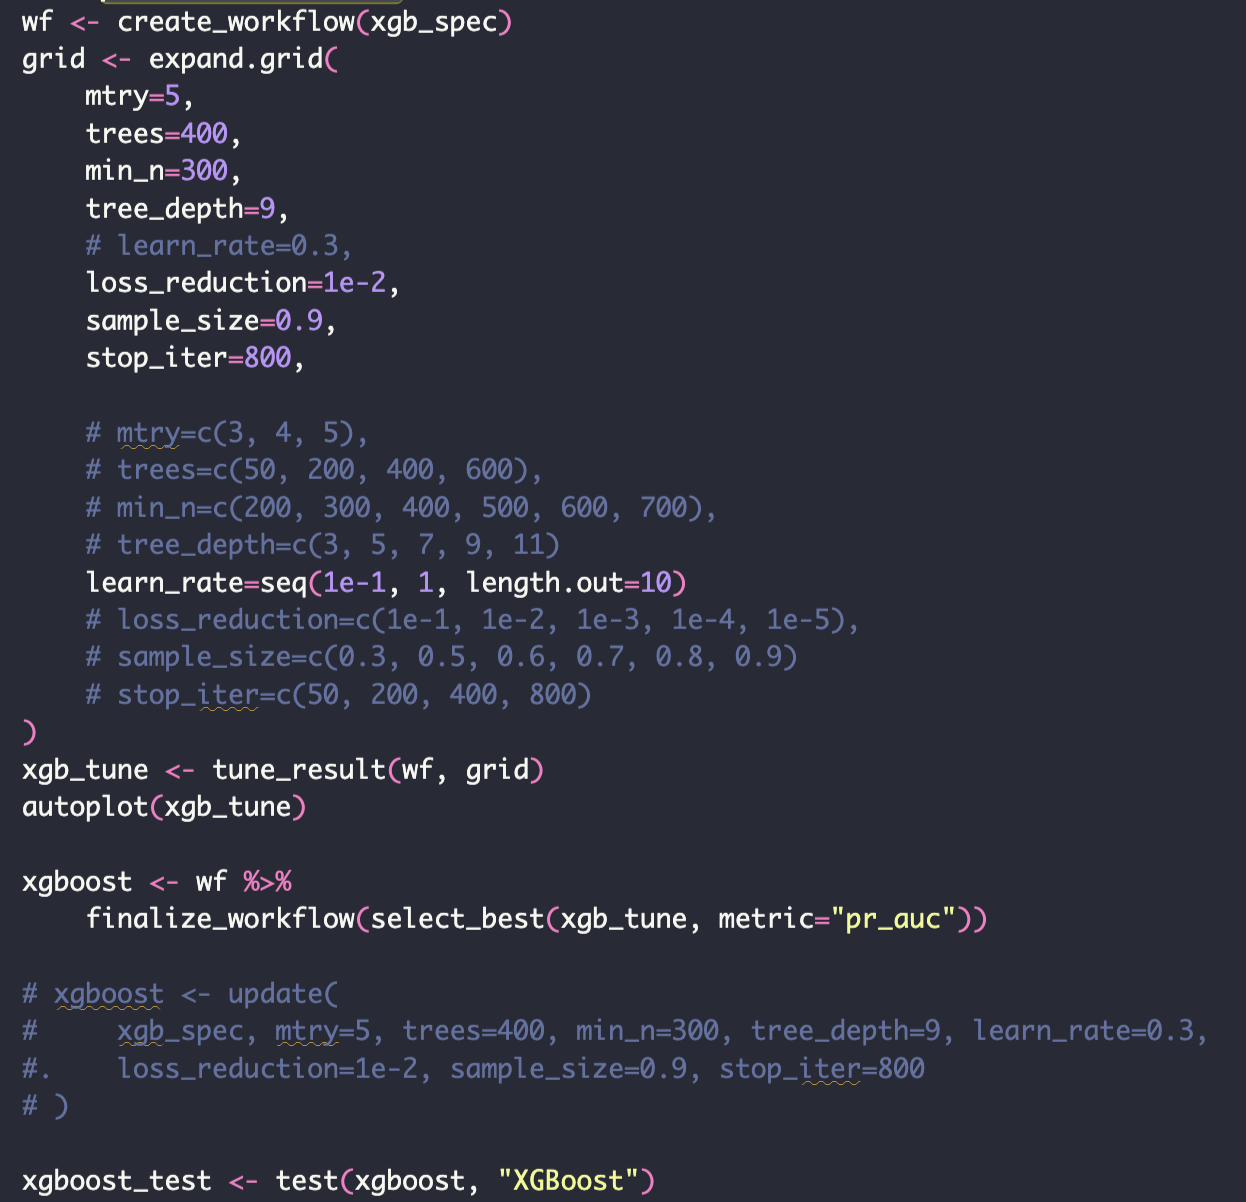
\includegraphics{figure/pdf/xgb2.png}
  \end{center}
\end{frame}


\begin{frame}{XGBoost}
  \begin{center}
    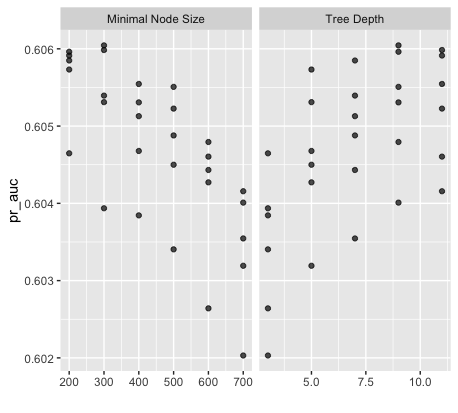
\includegraphics[width=0.7\textwidth]{figure/pdf/xgb_tune1.png}
  \end{center}
\end{frame}


\begin{frame}{AUPRC}
  \begin{center}
    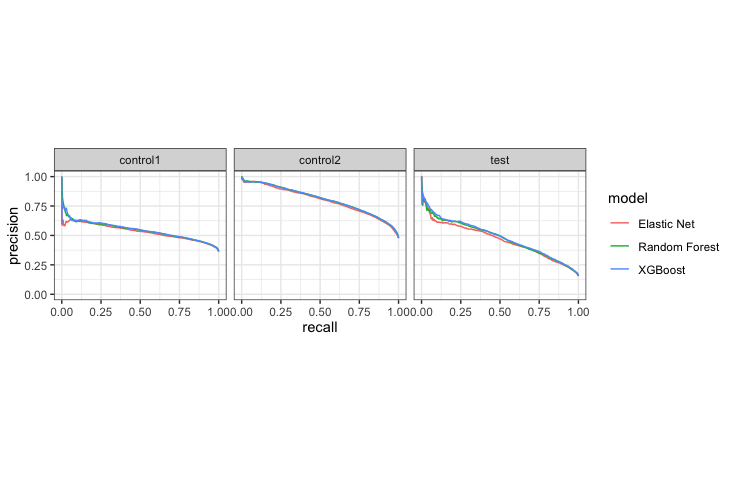
\includegraphics{figure/pdf/R_pr_curve.png}
  \end{center}
\end{frame}

\end{document}
